%!TEX root = draft.tex

\section{Discussion}
\label{sec:Discussion}
In this section, we discuss the insufficiency of the well-known triangle closing mechanism,
importance of measuring distributional network properties
and the limitations of our model \texttt{ARW}.

\subsection{Dissecting the Triangle Closing Mechanism}
\label{ss:tc}

Network models (e.g., \texttt{SAN} \cite{gong2012evolution} \& \texttt{HK} \cite{holme2002growing})
commonly use triangle closing mechanisms to generate networks with
varying average local clustering. However, our experimental results
in \cref{sub:Experimental Results} show that models that rely on triangle closing
cannot model the local clustering distribution or bivariate degree-clustering
relationship accurately. To understand why, we examine the degree-clustering
relationship in the \texttt{APS} network:
\vspace{-2mm}
\begin{figure}[H]
    \centering
    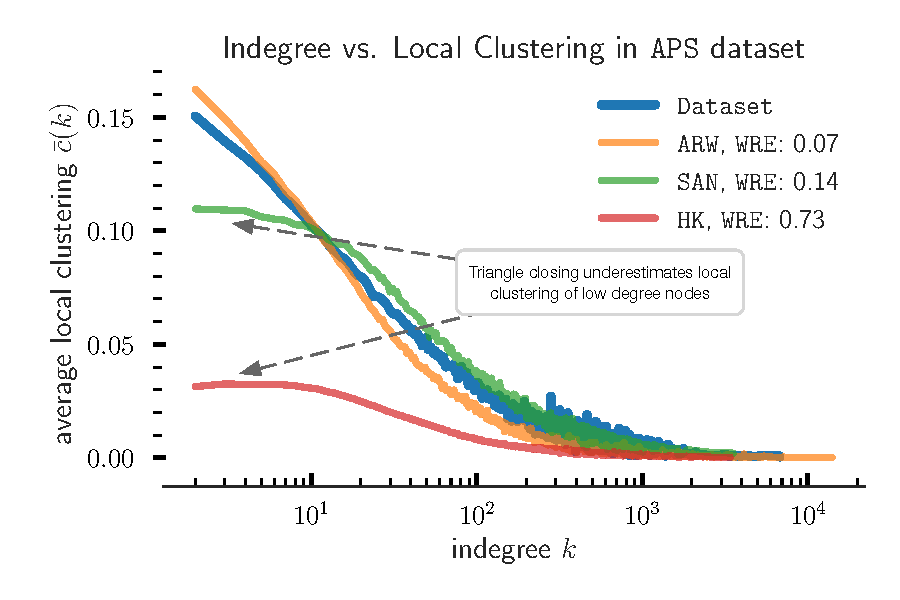
\includegraphics[width=.8\linewidth]{deg_cc_tc_om}
    \caption{Triangle closing mechanisms in \texttt{SAN} and \texttt{HK} fail to
    model average local clustering of low indegree nodes. In contrast, the random walk
    mechanism in \texttt{ARW} visits low indegree nodes and ``closes triangles'' in
    their neighborhoods to preserve local clustering with high accuracy.}
    \label{fig:triangle_closing}
\end{figure}

As annotated in \cref{fig:triangle_closing}, models based on triangle closing mechanisms,
\texttt{SAN} and \texttt{HK}, considerably underestimate the local clustering of
nodes that have low indegree. This is because incoming nodes in \texttt{SAN} and \texttt{HK}
tend to close triangles in the neighborhood of high indegree nodes to which they
connect via preferential attachment; Local clustering plateaus as indegree decreases because
triangle closing along with preferential attachment fail to form connections in neighborhoods
of low indegree nodes. In contrast, \texttt{ARW} accurately models the degree-clustering relationship
because incoming nodes initiate random walks in neighborhoods of seeds nodes that tend to have
low indegree.

\subsection{Measurement of Global Network Properties}
Despite their widespread usage, summary statistics of global
network properties such as global assortativity and average clustering have limited representative
power. Unlike point estimates, distributional properties reveal variance, skewness and anomalies
in network data.
Notably, understanding local processes via distributional network properties
guided the development of \texttt{ARW}, which consists of entirely \textit{local} processes
that do not rely on global information (e.g. fitness values of all nodes).
For instance, the \textit{skewed} clustering distribution and the relationship between clustering and
degree necessitated the jump parameter $p_j$ in our model. The structural constraints imposed by the jump
parameter amplify the effect of triadic closure and preserve high clustering
observed in neighborhoods of low degree nodes.
% Similarly, the variance in the
% local assortativity distribution of real-world networks necessitated additional
% stochasticity in the edge formation mechanism. As shown in
% \cref{subsec:LocalMixing}, \texttt{ARW} accurately models varying local mixing
% patterns because we augment seed selection to pick similar/dissimilar nodes
% probabilistically. As a result, incoming nodes with fixed preferences can
% initiate random walks in neighborhoods with varying local content properties.
To summarize, we believe that the analysis and evaluation of \textit{distributional}
network properties is crucial to accurately model network structure.


\subsection{\texttt{ARW} Limitations}
We discuss two limitations of our work. First, \texttt{ARW} does not preserve the average
path length distribution of real-world networks. This is because the random walk
mechanism is inherently local and does not form long-range connections to bridge
distant regions in the network. Preliminary experiments on forming ``structural bridges''
by initiating multiple random walks for every node indicate a tradeoff
between modeling small average path length and high local clustering. Second,
we only consider citation network datasets in order to study edge formation mechanisms of
incoming nodes that form all edges at once. We can adapt \texttt{ARW} to other
kinds of networks: attributed random walks that pause and resume intermittently
can jointly model edge formation processes between new and existing nodes in
social networks; Similarly, metapath based random walks can model interactions between
nodes of different types in heterogeneous information networks.
% In our future work, we plan to study the emergence of higher-order clustering
% \cite{yin2018higher} over time and the effect of homophily on the formation of
% temporal motifs \cite{paranjape2017motifs} via local processes such as \texttt{ARW}.

In this section, we first discussed the weaknesses of triangle closing mechanisms
and the importance of distributional network properties. Then, we briefly described
simple methods to extend \texttt{ARW} and address current limitations of our model.
%
% extend our model to incorporate the effect of multiple
% nto \texttt{ARW}
% to explain the emergence of higher-order clustering \cite{yin2018higher} and study
% the effect of homophily on the formation of temporal motifs \cite{paranjape2017motifs}.
% We believe that local processes such as random walks

% In this work, we address the problem of modeling growth of real-world
% bibliographic networks. Our proposed model is an improvement over existing
% random walk growth models that preserves multiple key network structural
% properties such as degree distribution, clustering coefficient distribution and their
% joint relationship. A standard modeling assumption is that \textit{new} nodes joining a
% network can potentially make connection to \textit{any} existing node in the network in
% some prescribed manner. Our experiments suggest that local link formation
% process in which \textit{new} nodes explore local network neighborhoods
% and makes connections in the explored locality can explain multiple structural
% properties of real-world networks.
%
% We note that clustering coefficient is an important characteristic of
% real-world networks. We observe that clustering is not
% uniformly distributed over the network and clustering at nodal level to be
% highly right skewed. The skewness implies that some parts of the network is more
% clustered than the other parts. In addition to skewness, clustering at nodal
% level is correlated to nodal degree. We propose a random-walk model the that
% gives rise to prominent characteristics of the network such as skewed local
% clustering.
%
% Finally, we show, via attributed network modeling, the extensibility
% of our proposed random walk model. The modeling suggests that our
% growth model can be adapted to account for growth of other kinds of
% information such as attributes and link types. Modeling other informative
% networks such as multiplex networks and heterogeneous information networks
% should be the focus of future work.

% \section{Limitations}
% Now, we discuss the limitations of our work. First, our work is limited to
% bibliographic datasets because of availibility of temporal data. We use the
% temporal out-degree sequence of incoming nodes in the network to model the
% network growth. In absence of temporal information, our growth model can be
% adapted by relying on the densification power law exponent. Second, our random
% walk model is sensitive to the initial graph. Since random walks explore the
% locality of a network and cannot access the entire network , the initial graph
% should have a giant weakly connected component. We recognise that the
% intialization problem can be addressed by having non-local source of information
% such as multiple seed nodes. Third, we note that our model fails to preserve
% certain network properties such as path length distribution. This is because
% our model does not account for nodes that serve as ``local bridges'' in the network.
% Modeling local and global processes simulatenously in a joint random walk model
% should lead to preservation of the discussed key network properties.
